% ============================================================
%  SCHOLA DOMESTICA — Magister Mathematica
%  Level 1 | Week 7 | Day 4
%  Topic: Addition — Mixed Practice, Sums to 10
%  (Word problems, missing addend intro, draw-and-count)
% ============================================================
\documentclass[12pt, letterpaper]{article}

\usepackage[top=1in, bottom=1in, left=1in, right=1in]{geometry}
\usepackage{fontenc}
\usepackage{inputenc}
\usepackage{lmodern}
\usepackage{microtype}
\usepackage{amsmath}
\usepackage{graphicx}
\usepackage{xcolor}
\usepackage{tikz}
\usepackage{array}
\usepackage{enumitem}
\usepackage{multicol}
\usepackage{mdframed}
\usepackage{fancyhdr}

\definecolor{scholared}{RGB}{160,30,30}
\definecolor{scholagold}{RGB}{180,140,40}
\definecolor{scholacream}{RGB}{253,248,235}
\definecolor{scholagreen}{RGB}{50,110,60}
\definecolor{scholablue}{RGB}{40,80,140}

\pagestyle{fancy}
\fancyhf{}
\renewcommand{\headrulewidth}{0.6pt}
\fancyhead[L]{\small\textcolor{scholared}{\textbf{Schola Domestica — Magister Mathematica}}}
\fancyhead[R]{\small\textcolor{scholared}{Level 1 · Week 7 · Day 4}}
\fancyfoot[C]{\small\textcolor{gray}{— \thepage\ —}}

\newcommand{\answerline}{\underline{\hspace{2.5cm}}}
\newcommand{\biganswerline}{\underline{\hspace{4cm}}}
\newcommand{\numbox}{\fbox{\hspace{0.6cm}\vphantom{0}}}

\newmdenv[
  backgroundcolor=scholacream,
  linecolor=scholared,
  linewidth=1.5pt,
  roundcorner=6pt,
  innertopmargin=8pt,
  innerbottommargin=8pt,
  innerleftmargin=10pt,
  innerrightmargin=10pt
]{lessonbox}

\begin{document}

\begin{center}
  {\LARGE\textbf{\textcolor{scholared}{Addition: Mixed Practice}}}\\[4pt]
  {\Large\textcolor{scholagold}{\textit{Sums to 10 — Facts and Stories}}}\\[6pt]
  {\small Name: \biganswerline \hspace{1cm} Date: \answerline}
\end{center}

\vspace{4pt}
\noindent\textcolor{scholared}{\rule{\linewidth}{1pt}}
\vspace{4pt}

% IMAGE PROMPT (Miyazaki-style watercolour):
% A cheerful open-air market stall overflowing with vegetables. A grandmother counts out
% 6 tomatoes from one basket and 4 from another into a large wooden bowl. Bright morning
% light, warm watercolour, farmers and children visible in background. No numerals.

% ===== PART I: FACTS =====
\noindent\textcolor{scholared}{\large\textbf{Part I — Addition Facts}} \hfill \textit{(Problems 1–10)}

\medskip\noindent\textit{Write the sum.}

\bigskip

\begin{multicols}{2}
\noindent\textbf{1.} $\; 5 + 2 = $ \numbox \\[10pt]
\noindent\textbf{2.} $\; 3 + 3 = $ \numbox \\[10pt]
\noindent\textbf{3.} $\; 6 + 1 = $ \numbox \\[10pt]
\noindent\textbf{4.} $\; 4 + 0 = $ \numbox \\[10pt]
\noindent\textbf{5.} $\; 2 + 8 = $ \numbox

\columnbreak

\noindent\textbf{6.} $\; 7 + 2 = $ \numbox \\[10pt]
\noindent\textbf{7.} $\; 0 + 0 = $ \numbox \\[10pt]
\noindent\textbf{8.} $\; 8 + 1 = $ \numbox \\[10pt]
\noindent\textbf{9.} $\; 4 + 6 = $ \numbox \\[10pt]
\noindent\textbf{10.} $\; 5 + 5 = $ \numbox
\end{multicols}

\bigskip
\noindent\textcolor{scholared}{\rule{\linewidth}{0.4pt}}

% ===== PART II: DRAW AND COUNT =====
\noindent\textcolor{scholared}{\large\textbf{Part II — Draw and Count}} \hfill \textit{(Problems 11–12)}

\medskip\noindent\textit{Draw circles to show each addition. Count all the circles. Write the sum.}

\bigskip
\noindent\textbf{11.} $4 + 3 =$ \numbox

\medskip
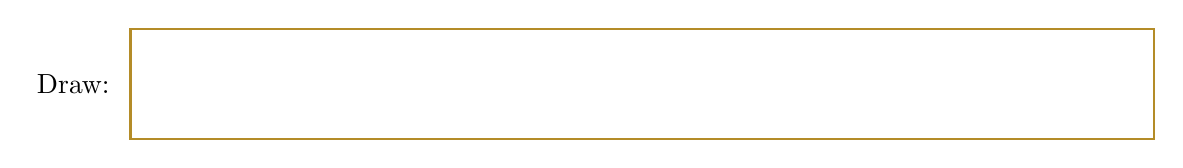
\begin{tikzpicture}
  \draw[thick, scholagold] (0,0) rectangle (13, 1.4);
  \node[left=4pt] at (0,0.7) {Draw:};
\end{tikzpicture}

\bigskip
\noindent\textbf{12.} $6 + 4 =$ \numbox

\medskip
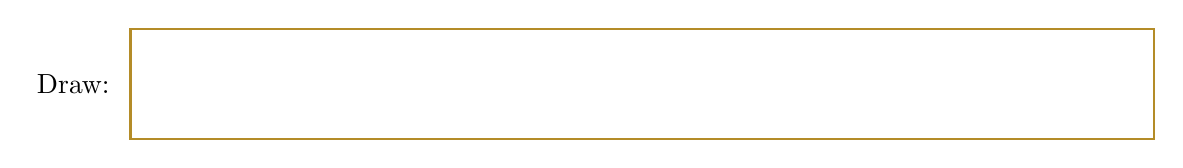
\begin{tikzpicture}
  \draw[thick, scholagold] (0,0) rectangle (13, 1.4);
  \node[left=4pt] at (0,0.7) {Draw:};
\end{tikzpicture}

\bigskip
\noindent\textcolor{scholared}{\rule{\linewidth}{0.4pt}}

% ===== PART III: WORD PROBLEMS =====
\noindent\textcolor{scholared}{\large\textbf{Part III — Word Problems}} \hfill \textit{(Problems 13–16)}

\bigskip
\noindent\textbf{13.} Thomas has 3 toy trains and 4 toy cars. How many toys in all?

\medskip
\hspace{2em} \numbox \; $+$ \; \numbox \; $=$ \; \numbox

\bigskip
\noindent\textbf{14.} A hen lays 6 eggs on Monday and 2 eggs on Tuesday. How many eggs?

\medskip
\hspace{2em} \numbox \; $+$ \; \numbox \; $=$ \; \numbox

\bigskip
\noindent\textbf{15.} Irene has 5 books and her brother has 5 books. How many books together?

\medskip
\hspace{2em} \numbox \; $+$ \; \numbox \; $=$ \; \numbox

\bigskip
\noindent\textbf{16.} There are 7 flowers in a vase. Nobody adds more. How many flowers?

\medskip
\hspace{2em} $7 + $ \numbox \; $=$ \; \numbox

\bigskip
\noindent\textcolor{scholared}{\rule{\linewidth}{0.4pt}}

% ===== PART IV: WHAT IS MISSING? =====
\noindent\textcolor{scholared}{\large\textbf{Part IV — What is Missing?}} \hfill \textit{(Problems 17–18)}

\medskip\noindent\textit{(Use the number line to help.)}

\bigskip
\noindent\textbf{17.} $4 + $ \numbox $= 6$ \hspace{2cm} \textbf{18.} $7 + $ \numbox $= 9$

\bigskip

\begin{center}
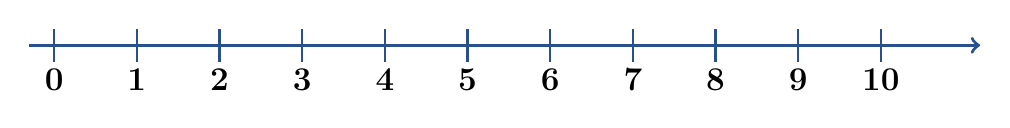
\begin{tikzpicture}[scale=1.05]
  \draw[very thick, scholablue, ->] (-0.3,0) -- (11.2,0);
  \foreach \n in {0,...,10} {
    \draw[thick, scholablue] (\n,0.2) -- (\n,-0.2);
    \node[below=5pt] at (\n,0) {\large\textbf{\n}};
  }
\end{tikzpicture}
\end{center}

\end{document}
